\documentclass{cours}
\usepackage{tkz-tab}

\title{Limites de Fonctions}

\begin{document}
    \maketitle{10}

    \begin{Gpartie}{Limites d'une Fonction en l'Infini} 
        \begin{Spartie}{Limite en $+\infty$} 
            \begin{SSpartie}{Définitions} 
                Soit une fonction $f$ définie au moins sur $\big[a~;+\infty\big[$, où $a$ est un réel.

                \begin{itemize}
                    \item   On dit que $f$ a pour limite $+\infty$ en $+\infty$ si pour tout réel $M$ positif, il existe un réel $A$, tel que $x>A$ implique $f(x)\geq M$. \\ Autrement dit, lorsque $x$ prend des valeurs de plus en plus grandes, $f(x)$ peut être aussi grand que l'on veut.
                    
                    On note : \[\lim\limits_{x\to +\infty}f(x)=+\infty\] 
                    \begin{center}
                        % \begin{tikzpicture}
                            \includegraphics[width=5cm]{example-image}
                        % \end{tikzpicture}
                        \parbox{\linewidth}{\captionof{figure}{\centering Représentation Graphique d'une Fonction qui Semble Tendre vers $+\infty$ en $+\infty$}}
                    \end{center}
                    \vspace*{2ex}
                    \item   On dit que $f$ a pour limite $-\infty$ en $+\infty$ si pout tout réel $m$ négatif, il existe un réel $A$, tel que $x>A$, $f(x)\leq m$. \\ Autrement dit, lorsque $x$ prend des valeurs de plus en plus grandes, $f(x)$ est négatif et peut être aussi grand que l'on veut en valeur absolue.
                    
                    On note : \[\lim\limits_{x\to +\infty}f(x)=-\infty\]
                    \begin{center}
                        % \begin{tikzpicture}
                            \includegraphics[width=5cm]{example-image}
                        % \end{tikzpicture}
                        \parbox{\linewidth}{\captionof{figure}{\centering Représentation Graphique d'une Fonction qui Semble Tendre vers $-\infty$ en $+\infty$}}
                    \end{center}
                    \vspace*{2ex}
                    \item   On dit que $f$ a pour limite $l$ en $+\infty$ où $l$ est un réel si pour tout intervalle ouvert $I$ contenant $l$, il existe un réel $A$ tel que $x>A$ implique $f(x)\in I$ \\ Autrement dit, lorsque $x$ prend des valeurs de plus en plus grandes, $f(x)$ peut être aussi près de $l$ que l'on veut.
                    
                    On note : \[\lim\limits_{x\to +\infty}f(x)=l\]
                    \begin{center}
                        % \begin{tikzpicture}
                            \includegraphics[width=5cm]{example-image}
                        % \end{tikzpicture}
                        \parbox{\linewidth}{\captionof{figure}{\centering Représentation Graphique d'une Fonction qui Semble Tendre vers $l$ en $+\infty$}}
                    \end{center}
                    \vspace*{2ex}
                    H.P.: $\forall\epsilon >0,~\exists A\in\mathbb{R},~\forall x\in\mathcal{D}_f$ \\ \phantom{H.P.: }$\bigg(x>A\implies\left\lvert f(x)-l\right\rvert <\epsilon\bigg)$ ou $\bigg(x>A\implies f(x)\in\big]l-\epsilon~;l+\epsilon\big[\bigg)$
                \end{itemize}
            \end{SSpartie}
            \begin{SSpartie}{Définition} 
                Soit $f$ une fonction définie au moins sur $\big[A~;+\infty\big[$, où $A$ est un réel, et $\mathcal{C}$ sa courbe représentative dans un repère. \\ Si $\lim\limits_{x\to+\infty}f(x)=l$ alors $\mathcal{C}$ admet une asymptote horizontale en $+\infty$ \\ d'équation $y=l$.
            \end{SSpartie}
            \begin{SSpartie}{Remarque} 
                Une fonction n'admet pas forcément de limite en $+\infty$, par exemple, les fonctions $\sin$ et $\cos$ sont bornées et n'admettent pas de limites en l'infini.
            \end{SSpartie}
        \end{Spartie}
        \begin{Spartie}{Limite en $-\infty$} 
            \begin{SSpartie}{Définitions}
                Soit $f$ une fonction définie au moins sur $\big]-\infty~;a\big[$, où $a$ est un réel.
                \begin{itemize}
                    \item   On dit que $f$ a pour limite $+\infty$ en $-\infty$ si pour tout réel $M$, positif, il existe un réel $A$ tel que $x<A$ implique $f(x)\geq M$ \\ Autrement dit, lorsque $x$ prend des valeurs négatives de plus en plus grandes en valeur absolue, $f(x)$ peut être aussi grand que l'on veut.
                    
                    On note : \[\lim\limits_{x\to-\infty}f(x)=+\infty\]
                    \begin{center}
                        % \begin{tikzpicture}
                            \includegraphics[width=5cm]{example-image}
                        % \end{tikzpicture}
                        \parbox{\linewidth}{\captionof{figure}{\centering Représentation Graphique d'une Fonction qui Semble Tendre vers $+\infty$ en $-\infty$}}
                    \end{center}
                    \vspace*{2ex}
                    \item   On dit que $f$ a pour limite $-\infty$ en $-\infty$ si pour tout réel $m$ négatif, il existe un réel $A$ tel que $x<A$ implique $f(x)\leq m$ \\ On note : \[\lim\limits_{x\to-\infty}f(x)=-\infty\]
                    \begin{center}
                        % \begin{tikzpicture}
                            \includegraphics[width=5cm]{example-image}
                        % \end{tikzpicture}
                        \parbox{\linewidth}{\captionof{figure}{\centering Représentation Graphique d'une Fonction qui Semble Tendre vers $-\infty$ en $-\infty$}}
                    \end{center}
                    \pagebreak
                    \item   On dit que $f$ a pour limite $l$ en $-\infty$ où $l$ est un réel, si pour tout intervalle ouvert $I$ contenant $l$, on peut trouver un réel $A$ tel que si $x\leq A$, $f(x)$ appartient à $I$. \\ Autrement dit, lorsque $x$ prend des valeurs négatives, de plus en plus grandes en valeur absolue, $f(x)$ peut être aussi près de $l$ que l'on veut.
                    
                    On note : \[\lim\limits_{x\to-\infty}f(x)=l\]
                    \begin{center}
                        % \begin{tikzpicture}
                            \includegraphics[width=5cm]{example-image}
                        % \end{tikzpicture}
                        \parbox{\linewidth}{\captionof{figure}{\centering Représentation Graphique d'une Fonction qui Semble Tendre vers $l$ en $+\infty$}}
                    \end{center}
                    \vspace*{2ex}
                    H.P.: $\forall\epsilon >0,~\exists A\in\mathbb{R},~\forall x\in\mathcal{D}_f$ \\ \phantom{H.P.: }$\bigg(x<A\implies\left\lvert f(x)-l\right\rvert <\epsilon\bigg)$ ou $\bigg(x<A\implies f(x)\in\big]l-\epsilon~;l+\epsilon\big[\bigg)$
                \end{itemize}
            \end{SSpartie}
            \begin{SSpartie}{Définition} 
                Si $\mathcal{C}$ est la courbe représentative de $f$ dans un repère. $\lim\limits_{x\to-\infty}f(x)=l$ alors $\mathcal{C}$ admet une asymptote horizontale en $-\infty$ d'équation $y=l$.
            \end{SSpartie}
        \end{Spartie}
    \end{Gpartie}
    \pagebreak
    \begin{Gpartie}{Limite d'une Fonction en un Réel} 
        \begin{Spartie}{Définitions} 
            Soit $a$ un réel et $f$ une fonction définie sur un intervalle $I$ contenant $a$ ou tel que $a$ est une borne de $I$.

            Si, lorsque $x$ prend des valeurs de plus en plus proches de $a$ :
            \begin{itemize}
                \item $f(x)$ est aussi grand que l'on veut, on dit que $f$ a pour limite $+\infty$ en $a$.

                On note : \[\lim\limits_{x\to a}f(x)=+\infty\]
                \begin{center}
                    % \begin{tikzpicture}
                        \includegraphics[width=5cm]{example-image}
                    % \end{tikzpicture}
                    \parbox{\linewidth}{\captionof{figure}{\centering Représentation Graphique d'une Fonction qui Semble Tendre vers $+\infty$ en $a$}}
                \end{center}
                \vspace*{2ex}
                \item $f(x)$ est négatif et aussi grand que l'on veut en valeur absolue, on dit que $f$ a pour limite $-\infty$ en $a$.

                On note : \[\lim\limits_{x\to a}f(x)=-\infty\]
                \begin{center}
                    % \begin{tikzpicture}
                        \includegraphics[width=5cm]{example-image}
                    % \end{tikzpicture}
                    \parbox{\linewidth}{\captionof{figure}{\centering Représentation Graphique d'une Fonction qui Semble Tendre vers $-\infty$ en $a$}}
                \end{center}
                \vspace*{2ex}
                \item $f(x)$ est aussi proche que l'on veut d'un réel $l$, on dit que $f$ a pour limite $l$ en $a$.
                
                On note : \[\lim\limits_{x\to a}f(x)=l\]
            \end{itemize}
            \begin{SSpartie}{Remarque} 
                Si $f$ est continue en $a$, $l=f(a)$.
            \end{SSpartie}
        \end{Spartie}
        \begin{Spartie}{Limite à Droite ou à Gauche d'une Fonction en un Réel} 
            \begin{SSpartie}{Exemple} 
                La fonction $f:x\mapsto\frac{1}{x}$ n'a pas de limite en $0$ car lorsque $x$ tend vers $0$ par des valeurs positives, $\frac{1}{x}$ tend vers $+\infty$ et lorsque $x$ tend vers $0$ par valeurs négatives, $\frac{1}{x}$ tend vers $-\infty$.

                Cependant, on peut parler de limite à gauche et limite à droite.

                On note : \[\lim\limits_{\substack{x\to 0 \\ x>0}}\frac{1}{x}=+\infty\qquad\lim\limits_{\substack{x\to 0 \\ x<0}}\frac{1}{x}=-\infty\]
            \end{SSpartie}
            \begin{SSpartie}{Remarque} 
                Une fonction admet une limite en un réel $a$ si la limite à droite et à gauche de $f$ en $a$ existent et sont égales.
            \end{SSpartie}
        \end{Spartie}
        \begin{Spartie}{Asymptote Verticale} 
            \begin{SSpartie}{Définition} 
                Soit $\mathcal{C}$ la courbe représentative de la fonction $f$. Dire que $\mathcal{C}$ admet une asymptote verticale d'équation $x=a$, c'est dire que : \[\lim\limits_{x\to a}f(x)=\pm\infty\quad\text{ou}\quad\lim\limits_{\substack{x\to a \\ x>a}}f(x)=\pm\infty\quad\text{ou}\quad\lim\limits_{\substack{x\to a \\ x<a}}f(x)=\pm\infty\]
            \end{SSpartie}
        \end{Spartie}
    \end{Gpartie}
    \pagebreak
    \begin{Gpartie}{Fonctions Usuelles} 
        \begin{Spartie}{Théorème} 
            \begin{SSpartie}{Fonction Racine Carrée} 
                $\lim\limits_{x\to+\infty}\sqrt{x}=+\infty$ et $\lim\limits_{x\to0}\sqrt{x}=0$ (la fonction racine carrée est continue en $0$)
            \end{SSpartie}
            \begin{SSpartie}{Fonction Inverse} 
                $\lim\limits_{x\to+\infty}\frac{1}{x}=0,\quad\lim\limits_{\substack{x\to a \\ x>a}}\frac{1}{x}=+\infty,\quad\lim\limits_{\substack{x\to a \\ x<a}}\frac{1}{x}=-\infty,\quad\lim\limits_{x\to-\infty}\frac{1}{x}=0$
            \end{SSpartie}
            \begin{SSpartie}{Fonctions Puissances} 
                Quel que soit $p\in\mathbb{N^*},~\lim\limits_{x\to+\infty}x^p=+\infty$

                Si $p$ est pair, $\lim\limits_{x\to-\infty}x^p=+\infty$ et si $p$ est impair, $\lim\limits_{x\to-\infty}=-\infty$
                
                \vspace*{2ex}Quel que soit $p\in\mathbb{N^*},~\lim\limits_{x\to+\infty}\frac{1}{x^p}=0$, et $\lim\limits_{x\to-\infty}\frac{1}{x^p}=0$

                Si $p$ est pair, $\lim\limits_{x\to0}\frac{1}{x^p}=+\infty$ et si $p$ est impair, $\lim\limits_{\substack{x\to0 \\ x>0}}\frac{1}{x^p}=+\infty$ et $\lim\limits_{\substack{x\to0 \\ x<0}}\frac{1}{x^p}=-\infty$
            \end{SSpartie}
            \begin{SSpartie}{Fonction Exponentielle} 
                $\lim\limits_{x\to+\infty}\me^x=+\infty,\quad\lim\limits_{x\to-\infty}\me^x=0$
            \end{SSpartie}
            \begin{SSpartie}{Fontion Logarithme Népérien} 
                $\lim\limits_{x\to+\infty}\ln(x)=+\infty,\quad\lim\limits_{\substack{x\to0 \\ x>0}}\ln(x)=-\infty$
            \end{SSpartie}
        \end{Spartie}
        \begin{Spartie}{Théorèmes de Croissance Comparée} 
            \[\lim\limits_{x\to+\infty}\frac{\me^x}{x}=+\infty\qquad\lim\limits_{x\to-\infty}x\me^x=0\]
            \begin{SSpartie}{Démonstration} 
                \begin{itemize}
                    \item On montre que $\me^x>\frac{x^2}{2}$, pour tout $x>0$ en étudiant la différence.

                    Soit $f$ définie sur $\big]0~;+\infty\big[$ par $f(x)=\me^x-\frac{x^2}{2}$. Étudions les variations de $f$.

                    $f'(x)=\me^x-x$ on ne conclut pas directement sur le signe. Dérivons encore :

                    $f''(x)=\me^x-1\quad\text{et}\quad \me^x-1>0\iff \me^x>1\iff x>0$

                    Donc, $f''(x)$ est strictement positive pour $x>0$

                    Ainsi on a $f'(x)$ strictement croissante sur $\big]0~;+\infty\big[$ et comme $f'(0)=1>0$, $f'$ est strictement positive sur $\big]0~;+\infty\big[$ :
                    \begin{center}                        
                        \vspace*{2ex}
                        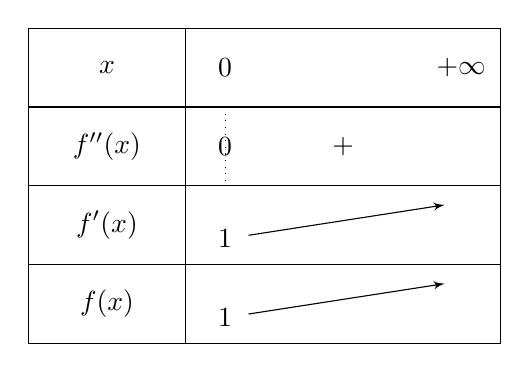
\begin{tikzpicture}
                            \tkzTabInit{$x$ /1, $f''(x)$ /1, $f'(x)$ /1, $f(x)$ /1}{$0$, $+\infty$}
                            \tkzTabLine{z,+,}
                            \tkzTabVar{-/$1$,+/}
                            \tkzTabVar{-/$1$,+/}
                        \end{tikzpicture}
                        \parbox{\linewidth}{\captionof{figure}{\centering Tableau de Variation de $f$}}
                        \vspace*{2ex}
                    \end{center}
                    Donc, pour tout $x\in\big]0~;+\infty\big[,~\me^x-\frac{x^2}{2}>0$ et donc $\me^x>\frac{x^2}{2}$ \\ Comme $x>0$ on peut diviser par $x$ : \\ Donc, $\frac{\me^x}{x}>\frac{x}{2}$ et comme $\lim\limits_{x\to+\infty}\frac{x}{2}=+\infty$, par comparaison : \[\lim\limits_{x\to+\infty}\frac{\me^x}{x}=+\infty\quad\square\]
                    \item On pose $X=-x$ et alors, $\lim\limits_{x\to-\infty}X=+\infty$ et $x\me^x=-X\me^{x}=-\frac{X}{\me^X}$
                    
                    Donc, par passage à l'inverse de la limite précédente : 
                    \[\lim\limits_{x\to-\infty}x\me^x=\lim\limits_{X\to+\infty}-\frac{X}{\me^X}=0\quad\square\]
                \end{itemize}
            \end{SSpartie}
        \end{Spartie}
        \begin{Spartie}{Théorème} 
            Quel que soit l'entier $n>0$ : \[\lim\limits_{x\to_\infty}\frac{\me^x}{x^n}=+\infty\quad\text{et}\quad\lim\limits_{x\to-\infty}x^n\me^x=0\]
        \end{Spartie}
        \begin{Spartie}{Théorèmes de Croissance Comparée (bis)} 
            \[\lim\limits_{x\to+\infty}\frac{\ln(x)}{x}=0\quad\text{et}\quad\lim\limits_{\substack{x\to0 \\ x>0}}x\ln(x)=0\]
            \begin{SSpartie}{Démonstration} 
                On pose le changement de variable $X=\ln(x)$ et donc $x=\me^X$. On a alors $\lim\limits_{x\to+\infty}X=+\infty$ et $\lim\limits_{\substack{x\to0 \\ x>0}}X=-\infty$.
            \end{SSpartie}
        \end{Spartie}
    \end{Gpartie}
    \begin{Gpartie}{Opérations sur les Limites} 
        \begin{Spartie}{Limites de Somme, Produit et Quotient} 
            Dans cette sous-partie, les limites des fonctions $f$ et $g$ sont prises soit en $-\infty$, soit en $+\infty$ soit en un réel $a$. $l$ et $l'$ sont des nombres réels. \\ Lorsqu'il n'y a pas de conclusion en général, on dit alors qu'il y a un cas de forme indéterminée. (F.I.) \\
            N.B.: $\pm\infty$ désigne $+\infty$ ou $-\infty$.
            \begin{SSpartie}{Limite de Somme} 
                \begin{center}\begin{tabular}{ |m{0.15\linewidth}||*{6}{>{\centering\arraybackslash}m{0.1\linewidth}| }} \hline
                    Si $\lim f$     & $l$   & $l$       & $l$       & $+\infty$ & $-\infty$ & $+\infty$ \\\hline
                    Si $\lim g$     & $l'$  & $+\infty$ & $-\infty$ & $+\infty$ & $-\infty$ & $-\infty$ \\\hline
                    $\lim (f+g)$    & $l+l'$& $+\infty$ & $-\infty$ & $+\infty$ & $-\infty$ & F.I.      \\\hline
                \end{tabular}\end{center}
                \parbox{\linewidth}{\captionof{figure}{\centering Tableau des Limites de Sommes de Fonctions}}
            \end{SSpartie}
            \begin{SSpartie}{Limite d'un Produit} 
                \begin{center}\begin{tabular}{ |m{0.13\linewidth}||*{9}{>{\centering\arraybackslash}m{0.06\linewidth}| }} \hline
                    Si $\lim f$         & $l$           & $l>0$     & $l>0$     & $l<0$     & $l<0$     & $+\infty$ & $+\infty$ & $-\infty$ & $0$ \\\hline
                    Si $\lim g$         & $l'$          & $+\infty$ & $-\infty$ & $+\infty$ & $-\infty$ & $+\infty$ & $-\infty$ & $-\infty$ & $\pm\infty$ \\\hline
                    $\lim (f\times g)$  & $l\times l'$  & $+\infty$ & $-\infty$ & $-\infty$ & $+\infty$ & $+\infty$ & $-\infty$ & $-\infty$ & F.I. \\\hline
                \end{tabular}\end{center}
                \parbox{\linewidth}{\captionof{figure}{\centering Tableau des Limites des Produits de Fonctions}}
            \end{SSpartie}
            \begin{SSpartie}{Limite d'un Quotient $f/g$ dans le cas où la limite de $g$ n'est pas nulle} 
                \begin{center}\begin{tabular}{ |m{0.15\linewidth}||*{7}{>{\centering\arraybackslash}m{0.082\linewidth}| }} \hline
                    Si $\lim f$     & $l$           & $l$           & $+\infty$ & $+\infty$ & $-\infty$ & $-\infty$ & $\pm\infty$ \\\hline
                    Si $\lim g$     & $l'\neq0$     & $\pm\infty$   & $l'>0$    & $l'<0$    & $l'>0$    & $l'<0$    & $\pm\infty$ \\\hline
                    $\lim (f/g)$    & $\frac{l}{l'}$& $0$           & $+\infty$ & $-\infty$ & $-\infty$ & $+\infty$ & F.I. \\\hline
                \end{tabular}\end{center}
                \parbox{\linewidth}{\captionof{figure}{\centering Tableau des Limites des Quotients de Fonctions, où la Limite de $g$ n'est pas nulle}}
            \end{SSpartie}
            \pagebreak
            \begin{SSpartie}{Limite d'un Quotient $f/g$ dans le cas où la limite de $g$ est nulle} 
                \begin{center}\begin{tabular}{ |m{0.15\linewidth}||*{5}{>{\centering\arraybackslash}m{0.1\linewidth}| }} \hline
                    Si $\lim f$ & $l>0$ ou $+\infty$    & $l>0$ ou $+\infty$    & $l<0$ ou $-\infty$    & $l<0$ ou $-\infty$    & $0$ \\\hline
                    Si $\lim g$ & $0^+$                 & $0^-$                 & $0^+$                 & $0^-$                   & $0$ \\\hline
                    $\lim (f/g)$& $+\infty$           & $-\infty$           & $-\infty$           & $+\infty$               & F.I. \\\hline
                \end{tabular}\end{center}
                \parbox{\linewidth}{\captionof{figure}{\centering Tableau des Limites des Quotients de Fonctions, où la Limite de $g$ est nulle}}
            \end{SSpartie}
            \begin{SSpartie}{Exemples} 
                \begin{SSSpartie}{Somme} 
                    $\lim\limits_{x\to+\infty}x+\dfrac{1}{x^2}-1=+\infty$\quad(remarquons qu'on a la même limite quand $x\to0$)
                \end{SSSpartie}
                \begin{SSSpartie}{Produit} 
                    $\lim\limits_{x\to0}\left(-3+x\right)\left(1+\frac{1}{x^2}\right)=-\infty$\qquad En effet, $\lim\limits_{x\to0}-3+x=-3$ et $\lim\limits_{x\to0}1+\frac{1}{x^2}=+\infty$
    
                    Par contre, remarquons que $\lim\limits_{x\to+\infty}\left(-3+x\right)\left(1+\frac{1}{x^2}\right)=+\infty$
                \end{SSSpartie}
                \begin{SSSpartie}{Quotient} 
                    $\lim\limits_{x\to0}\dfrac{1+x}{\sqrt{x}}=+\infty$
                \end{SSSpartie}
            \end{SSpartie}
        \end{Spartie}
        \pagebreak
        \begin{Spartie}{Limite d'une Composée de Deux Fonctions} 
            \begin{SSpartie}{Rappel} 
                On note $g\circ f$ la composée de la fonction $f$ suivie de $g$.

                $\forall x\in\mathcal{D}_f$ tel que $f(x)\in\mathcal{D}_g,~(g\circ f)(x)=g\big(f(x)\big)$
            \end{SSpartie}
            \begin{SSpartie}{Théorème} 
                Soient $a$, $b$ et $c$ trois réels ou $+\infty$ ou $-\infty$. Soient $f$ et $g$ deux fonctions, définies au bon endroit. 
                
                Alors, si $\lim\limits_{x\to a}f(x)=\boldsymbol{b}$\quad et\quad$\lim\limits_{x\to\boldsymbol{b}}g(x)=c$, on a : \[\lim\limits_{x\to a}(g\circ f)(x)=c\]
                Attention aux limites !
            \end{SSpartie}
            \begin{SSpartie}{Exemple} 
                $\lim\limits_{x\to+\infty}\me^{-x^2-3}=0\quad$ car $\quad\lim\limits_{x\to+\infty}-x^2-3=-\infty\quad$ et $\quad\lim\limits_{X\to-\infty}\me^X=0$
            \end{SSpartie}
        \end{Spartie}
        \begin{Spartie}{Comparaison} 
            $a$ désigne un réel ou $+\infty$ ou $-\infty$.
            \begin{SSpartie}{Théorème} 
                Si $f$ et $g$ sont deux fonctions telles que pour tout $x$ voisin de $a$, $f(x)\leq g(x)$
                \begin{itemize}
                    \item Si $\lim\limits_{x\to a}f(x)=+\infty\quad$ alors $\quad\lim\limits_{x\to a}g(x)=+\infty$
                    \item Si $\lim\limits_{x\to a}g(x)=-\infty\quad$ alors $\quad\lim\limits_{x\to a}f(x)=-\infty$
                \end{itemize}
            \end{SSpartie}
            \begin{SSpartie}{Théorème} 
                Soient $f$, $g$ et $h$ trois fonctions telles que pour tout $x$ voisin de $a$, $g(x)\leq f(x)\leq h(x)$

                Si $\lim\limits_{x\to a}g(x)=l\quad$ et $\quad\lim\limits_{x\to a}h(x)=l\quad$ où $l$ est un réel, alors $\quad\lim\limits_{x\to a}f(x)=l$
            \end{SSpartie}
        \end{Spartie}
    \end{Gpartie}
\end{document}